\documentclass[11pt]{article}
\usepackage[a4paper,margin=26mm]{geometry}
\usepackage[T1]{fontenc}
\usepackage{lmodern}
\usepackage{amsmath,amssymb,amsthm}
\usepackage{microtype}
\usepackage{array}
\usepackage{tikz}
\usepackage{xurl}
\usepackage{hyperref}
\hypersetup{colorlinks=true,linkcolor=blue,urlcolor=blue,citecolor=blue,
 pdftitle={A Lean-verified strict edge net for crossed polygonal roofs over a parallelogram},
 pdfauthor={Horace Dong}}
\newtheorem{theorem}{Theorem}
\newtheorem{lemma}{Lemma}
\newtheorem{proposition}{Proposition}
\newtheorem{corollary}{Corollary}
\theoremstyle{definition}
\newtheorem{definition}{Definition}
\theoremstyle{remark}
\newtheorem{remark}{Remark}
\newcommand{\repoversion}{1.26.0}
\setlength{\emergencystretch}{1.5em}
\newcommand{\R}{\mathbb R}
\newcommand{\cR}{\mathcal R}
\newcommand{\cF}{\mathcal F}

\title{A Lean-verified strict edge net for crossed\\ polygonal roofs over a parallelogram}
\author{Horace Dong\\ \small Independent researcher\\
\small\texttt{maxwelldhx@gmail.com}\\
\small ORCID: \href{https://orcid.org/0009-0002-7554-7548}{0009-0002-7554-7548}}
\date{23 November 2026}
\begin{document}
\sloppy
\maketitle

\begin{abstract}
We give an explicit edge unfolding for a special family of convex polyhedra:
the vertical projection is a parallelogram, the top is a concave polygonal
roof whose ridges are parallel to one side of the parallelogram, the bottom
is a convex polygonal floor whose ridges are parallel to the other side, and
the numbers of roof and floor facets are arbitrary. Every facet is placed isometrically, and two surface points have the
same image only if they are the same point glued along uncut edges; so the
unfolding is a strict net, without overlap and without boundary contact
beyond the hinges. These two statements and an oblique example are verified in
Lean~4 in coordinate form; the facet structure, the cut tree and the disk
topology are argued in the text. The construction is elementary and
does not use convexity; for a rectangular projection a net was known to exist
by a theorem of O'Rourke. This is not a step towards D\"urer's problem in
general. The proofs were found and formalized by AI
agents working under the author's direction; their role is described at the
end of the paper.
\end{abstract}

\section{Introduction}\label{sec:intro}

The question ``Can every convex polyhedron be cut along its edges and
unfolded flat to a single, nonoverlapping, simple polygon?'' is Problem~9 of
The Open Problems Project~\cite{topp}. It was first stated by
Shephard~\cite{shephard}, and in spirit it goes back to Albrecht D\"urer
(1525); it is open~\cite{topp}. Such an unfolding is called a \emph{net}.
The classes of convex polyhedra known to have edge unfoldings to nets are
listed in~\cite[Section~22.5]{do07} and in the update~\cite{do25} of
September 2025 (among them prismoids, domes, affine
stretchings~\cite{ghomi}, tall or rectangular-base prismatoids~\cite{bdm},
polyhedra with a Hamiltonian
quasigeodesic~\cite{oro22}, nested prismatoids~\cite{radons} and tapered
polyhedra). In~\cite{do25} a net may touch itself on the boundary;
only overlap of interior points is excluded. Recent work~\cite{mit26} on
overlapping edge unfoldings does not settle the problem.

\paragraph{The result.} Let $\Pi$ be a parallelogram in the horizontal plane
with sides parallel to unit vectors $u$ and $v$. A \emph{crossed-roof solid}
(Section~\ref{sec:family}) lies over $\Pi$ between a roof and a floor: the
roof is the graph of a concave piecewise linear function of the
$u$-coordinate alone, so its ridges are parallel to $v$; the floor is the
graph of a convex piecewise linear function of the $v$-coordinate alone, so
its ridges are parallel to $u$; the roof is strictly above the floor. There
are four vertical walls and any numbers $n,m\ge1$ of roof and floor facets.
We give an explicit edge unfolding of every crossed-roof solid
(Figure~\ref{fig:net}) and prove that it is a \emph{strict} net, with no
boundary contact beyond the hinges. The metric and contact statements are formally verified in
Lean~4 for the whole family (Theorem~\ref{thm:main}), with an explicit oblique
member (Theorem~\ref{thm:example}).

\paragraph{What this is and what it is not.} This is a special case, not
progress on the general problem. Every facet is parallel to $u$ or to $v$; the
roof and the floor each unroll to a monotone strip attached to the band of
walls. The argument does not use
convexity (Remark~\ref{rem:convexity}). For a rectangular $\Pi$ a net (with
boundary contact allowed) exists by O'Rourke's
theorem~\cite[Theorem~1]{oro22}, since these solids have a Hamiltonian
quasigeodesic (Section~\ref{sec:prior}); there only the strictness of this
particular net is added. For oblique $\Pi$ we show for one example that
\cite{oro22} does not apply; we have not shown this for every oblique member.
Members with $n=1$ or $m=1$ are prismatoids (Section~\ref{sec:prior}). The
searches described at the end found no published edge-unfoldable class
containing the oblique members with $n,m\ge2$; we make no further claim of
novelty.

\section{The family}\label{sec:family}

\begin{definition}[profile]\label{def:profile}
A \emph{profile} of length $a>0$ with $n\ge1$ pieces consists of knots
$0=t_0<t_1<\dots<t_n=a$, slopes $\mu_0,\dots,\mu_{n-1}\in\R$ and a function
$f$ on $[0,a]$ such that for every $i<n$ and every $t\in[0,a]$
\[
f(t)\le f(t_i)+\mu_i(t-t_i),\qquad\text{with equality if and only if } t_i\le t\le t_{i+1}.
\]
\end{definition}

\noindent So $f$ is the minimum of $n$ affine functions, each tight exactly
on its own piece: $f$ is concave, piecewise linear, and bends at every interior
knot.

\begin{definition}[crossed-roof solid]\label{def:solid}
Let $f$ be a profile of length $a$ with $n$ pieces and slopes $\mu_i$, let
$h$ be a profile of length $b$ with $m$ pieces and slopes $\nu_j$, put
$g=-h$ (a convex function on $[0,b]$), and let $-1<c\le0$. Assume
$g(y)<f(x)$ for all $x\in[0,a]$, $y\in[0,b]$. Let $u,v$ be horizontal unit
vectors with $u\cdot v=c$ and $e_3$ the vertical unit vector; the point with
coordinates $(x,y,z)$ is $xu+yv+ze_3$. The solid is
\[
P=\{(x,y,z):\ 0\le x\le a,\ 0\le y\le b,\ g(y)\le z\le f(x)\}.
\]
\end{definition}

\noindent In Cartesian coordinates, $(x,y,z)$ is the point
$E(x,y,z)=(x+cy,\ \sqrt{1-c^2}\,y,\ z)$, so
\begin{equation}\label{eq:gram}
|E(p)-E(q)|^2=\Delta x^2+2c\,\Delta x\,\Delta y+\Delta y^2+\Delta z^2 .
\end{equation}
The boundary of $P$ consists of the six closed \emph{charts}
\[
\text{roof } z=f(x),\quad A: x=0,\quad B: y=b,\quad C: x=a,\quad D: y=0,\quad \text{floor } z=g(y)
\]
(each intersected with $P$), in this order; the walls $A,B,C,D$ are in
cyclic order around $\Pi$. The roof is divided into the facets
$\cR_i=\{t_i\le x\le t_{i+1}\}$, $i<n$, and the floor into the facets
$\cF_j$, $j<m$, given by the knots of $h$.

\paragraph{The sign of $c$ (written argument).} The condition $c\le0$ means
that the corner at the origin of $\Pi$ is obtuse or right. This is no loss of
generality: if $0<c<1$, replace $x$ by $a-x$ (that is, $u$ by $-u$ and the
corner at the origin by the adjacent one). This changes $c$ into $-c$,
replaces the roof function by $x\mapsto f(a-x)$, which is again a concave
profile, and leaves the floor unchanged. This reduction is not formalized.

\section{The net}\label{sec:net}

For a slope $\mu$ let $k(\mu)=\sqrt{1+\mu^2-c^2}$, which is positive since
$c^2<1$. Let $U$ be the continuous piecewise linear function on $[0,a]$ with
$U(0)=0$ and slope $k(\mu_i)$ on $[t_i,t_{i+1}]$, and let $V$ be the
analogous function on $[0,b]$ built from the slopes $\nu_j$; both are
strictly increasing. With $w=2a+2b$ (the perimeter of $\Pi$), the planar
maps of the six charts are
\begin{align*}
\text{roof}:&\ (x,y,z)\mapsto(y+cx,\ f(0)+U(x)), &
A:&\ (y,\ z), & B:&\ (b+x,\ z),\\
\text{floor}:&\ (x,y,z)\mapsto(w-x-cy,\ g(0)-V(y)), &
C:&\ (2b+a-y,\ z), & D:&\ (w-x,\ z).
\end{align*}
The walls are laid out in a row in the order $A,B,C,D$; the roof is hinged to
the top edge of $A$ and the floor to the bottom edge of $D$
(Figure~\ref{fig:net}). These two edges, $A\cap B$, $B\cap C$, $C\cap D$ and all
ridges inside the roof and the floor are kept as hinges; all other edges are
cut.

\begin{theorem}[formally verified]\label{thm:main}
For every crossed-roof solid there are functions $U$ and $V$ with
$U(0)=V(0)=0$, strictly increasing on $[0,a]$ and on $[0,b]$, such that
$U(x)-U(x')=k(\mu_i)(x-x')$ for $x,x'\in[t_i,t_{i+1}]$ and
$V(y)-V(y')=k(\nu_j)(y-y')$ for $y,y'$ in the $j$-th piece of $h$ (on
$[0,a]$ and $[0,b]$ these conditions determine the functions $U$ and $V$
above), and such that, for the planar maps $\Phi_K$ of the charts $K$
defined with them:
\begin{enumerate}
\item[(i)] \emph{(isometry)} if $p,q$ lie on the same chart $K$, and in the
same roof facet $\cR_i$ when $K$ is the roof, or in the same floor facet
$\cF_j$ when $K$ is the floor, then $|\Phi_K(p)-\Phi_K(q)|=|E(p)-E(q)|$;
\item[(ii)] \emph{(contacts)} if $p$ lies on the chart $K$ and $q$ on the
chart $L$, then $\Phi_K(p)=\Phi_L(q)$ if and only if $p=q$ and $p$ lies on
every chart between $K$ and $L$ in the order roof, $A$, $B$, $C$, $D$, floor.
\end{enumerate}
\end{theorem}

\noindent The points in~(i) and~(ii) are arbitrary points of the closed
charts, boundary included; $K=L$ in~(ii) gives injectivity of each chart map.
For instance, a point of the cut edge $A\cap D$ is not on $B$, so its copies
on $A$ and $D$ have different images, while the corner $(0,b,f(0))$ lies on
the roof, $A$ and $B$, so its images in the roof and in $B$ coincide.

\begin{theorem}[formally verified]\label{thm:example}
There is a crossed-roof solid with $c=-\tfrac12$, $a=b=2$, $n=m=2$,
$f(t)=\min\{3,\ 3+(1-t)/10\}$ and $g(t)=\max\{0,\ (t-1)/10\}$ for
$t\in[0,2]$.
\end{theorem}

\begin{figure}[!htbp]
\centering
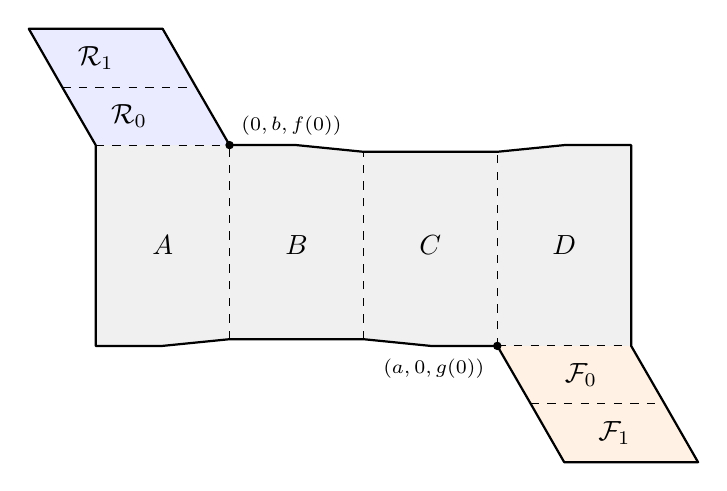
\begin{tikzpicture}[scale=0.85,line join=round]
\tikzset{hinge/.style={draw=black,dashed,thin}}
\fill[gray!12] (0,0)--(1,0)--(2,0.1)--(2,3)--(0,3)--cycle;
\fill[gray!12] (2,0.1)--(4,0.1)--(4,2.9)--(3,3)--(2,3)--cycle;
\fill[gray!12] (4,0.1)--(5,0)--(6,0)--(6,2.9)--(4,2.9)--cycle;
\fill[gray!12] (6,0)--(8,0)--(8,3)--(7,3)--(6,2.9)--cycle;
\fill[blue!8] (0,3)--(-0.5,3.866)--(-1,4.738)--(1,4.738)--(1.5,3.866)--(2,3)--cycle;
\fill[orange!10] (6,0)--(6.5,-0.866)--(7,-1.738)--(9,-1.738)--(8.5,-0.866)--(8,0)--cycle;
\draw[thick] (0,3)--(0,0)--(1,0)--(2,0.1)--(4,0.1)--(5,0)--(6,0)--(6.5,-0.866)
 --(7,-1.738)--(9,-1.738)--(8.5,-0.866)--(8,0)--(8,3)--(7,3)--(6,2.9)--(4,2.9)
 --(3,3)--(2,3)--(1.5,3.866)--(1,4.738)--(-1,4.738)--(-0.5,3.866)--cycle;
\draw[hinge] (0,3)--(2,3);
\draw[hinge] (-0.5,3.866)--(1.5,3.866);
\draw[hinge] (2,0.1)--(2,3);
\draw[hinge] (4,0.1)--(4,2.9);
\draw[hinge] (6,0)--(6,2.9);
\draw[hinge] (6,0)--(8,0);
\draw[hinge] (6.5,-0.866)--(8.5,-0.866);
\fill (2,3) circle (1.8pt);
\fill (6,0) circle (1.8pt);
\node at (1,1.5) {$A$};
\node at (3,1.5) {$B$};
\node at (5,1.5) {$C$};
\node at (7,1.5) {$D$};
\node at (0.5,3.43) {$\cR_0$};
\node at (0,4.3) {$\cR_1$};
\node at (7.25,-0.43) {$\cF_0$};
\node at (7.75,-1.3) {$\cF_1$};
\node[font=\scriptsize,anchor=south west] at (2.03,3.0) {$(0,b,f(0))$};
\node[font=\scriptsize,anchor=north east] at (5.95,-0.05) {$(a,0,g(0))$};
\end{tikzpicture}
\caption{The net of the solid of Theorem~\ref{thm:example} ($a=b=2$,
$c=-\frac12$), from the maps of Section~\ref{sec:net} ($A$ spans $0\le s\le2$,
$D$ spans $6\le s\le8$). Dashed: kept edges (hinges); solid: cut edges. Faces
not adjacent along a hinge meet only at the two dots, the images of the
corners $(0,b,f(0))$ and $(a,0,g(0))$, single points of the polyhedron glued
through the walls. As $c<0$, the roof is sheared left and the floor right.}
\label{fig:net}
\end{figure}

\begin{proof}[Written proof of Theorem~\ref{thm:main}]
\emph{Isometry.} Each wall map is an isometry of its plane: on $A$ and $C$
we have $\Delta x=0$ and on $B$ and $D$ we have $\Delta y=0$, so
by~\eqref{eq:gram} the spatial distance is $\sqrt{\Delta y^2+\Delta z^2}$ or
$\sqrt{\Delta x^2+\Delta z^2}$, which is the planar distance. On a roof facet
$\cR_i$ we have $\Delta z=\mu_i\Delta x$, and the planar displacement is
$(\Delta y+c\Delta x,\ k(\mu_i)\Delta x)$, whose squared length is
\[
(\Delta y+c\Delta x)^2+(1+\mu_i^2-c^2)\Delta x^2
=\Delta x^2+2c\,\Delta x\,\Delta y+\Delta y^2+\mu_i^2\Delta x^2 ,
\]
the right-hand side of~\eqref{eq:gram}. The floor is the same computation with
$x$ and $y$ exchanged.

\emph{Images.} Write $(s,\eta)$ for planar coordinates. Since $c\le0$ and
$x,y\ge0$:
the roof image lies in $\{s\le b,\ \eta\ge f(0)\}$, with $\eta=f(0)$ only for
$x=0$; $A$ lies in $\{0\le s\le b,\ \eta\le f(0)\}$; $B$ in $\{b\le s\le a+b\}$;
$C$ in $\{a+b\le s\le a+2b\}$; $D$ in $\{a+2b\le s\le w\}$; and the floor
image lies in $\{s\ge w-a,\ \eta\le g(0)\}$, with $s=w-a$ only for $x=a$
and $cy=0$, and $\eta=g(0)$ only for $y=0$.

\emph{Contacts.} If two points are glued as in~(ii), the formulas agree on the common edges (for example, on the edge
between the roof and $A$, $x=0$ and $z=f(0)$, and both maps give $(y,f(0))$),
so their images coincide. Conversely, suppose $\Phi_K(p)=\Phi_L(q)$. Within
the roof, $\eta$ determines $x$ because $U$ is strictly increasing, and then
$s$ determines $y$; similarly for the floor, and the wall maps are injective,
so $K=L$ forces $p=q$. Walls that are not consecutive in the row have disjoint
$s$-ranges; in particular $A$ ($s\le b$) and $D$ ($s\ge a+2b$) never meet,
which is the cut edge $A\cap D$. Consecutive walls meet only on the line
$s=b$, $s=a+b$ or $s=a+2b$, where both maps describe the same vertical edge
with the same height range. The roof meets $A$ only where $\eta=f(0)$, so
$x=0$, which is the hinge. The roof meets $B$ only on $s=b$, which forces
$y=b$ and $cx=0$; there $B$ has heights at most $f(0)$ (its top at $x=0$),
so $\eta=f(0)$, hence $x=0$, and the common point is the corner $(0,b,f(0))$,
which lies on the roof, $A$ and $B$. The roof is disjoint from $C$, $D$ and
the floor, since $b<a+b$. Symmetrically, the floor meets $D$ only along the
hinge $y=0$, meets $C$ only at the corner $(a,0,g(0))$, which lies on $C$, $D$
and the floor, and is disjoint from $A$ and $B$.
\end{proof}

\begin{remark}[convexity is not used]\label{rem:convexity}
The proof uses the affine form of $f$ and $g$ on each piece, the positivity of
the rates $k(\mu)$, the bounds $g(y)\le z\le f(x)$ and $c\le0$, but not the
inequalities that make $f$ concave and $g$ convex, nor the gap $g<f$; the Lean
proof files do not refer to the support inequality, the gap or the covering
condition either. Convexity is needed only to know that $P$ is a convex
polyhedron with the facets described below. The restriction $c\le0$ only
shortens the separation argument; the same maps also appear to work for
$0<c<1$, but we neither prove nor use this.
\end{remark}

\paragraph{The polyhedron and its net (written argument, not formalized).}
$P$ is the intersection of the halfspaces below the $n$ supporting planes of
the roof, above the $m$ supporting planes of the floor, and the four wall
halfspaces; it is bounded with interior points, hence a convex polyhedron.
Each of these $n+m+4$ planes meets $P$ in a polygon with interior (pieces
have positive length and $g<f$), and consecutive slopes differ, so the facets
are exactly $\cR_0,\dots,\cR_{n-1}$, $\cF_0,\dots,\cF_{m-1}$, $A$, $B$, $C$,
$D$; $P$ has $2(n+m+2)$ vertices. The kept edges join the facets in the path
$\cR_{n-1},\dots,\cR_0,A,B,C,D,\cF_0,\dots,\cF_{m-1}$, a spanning tree of the
dual graph, so the cut edges form a spanning tree of the $1$-skeleton, in fact
a Hamiltonian path: the three sides of the roof other than its hinge with $A$,
from $(0,b)$ to $(0,0)$; the vertical edge $A\cap D$; and the three sides of
the floor other than its hinge with $D$, from $(0,0)$ to $(a,0)$. Attaching
the facets one at a time, each along one full edge, gives a closed polygonal
disk, the cut surface. By Theorem~\ref{thm:main} the planar map is well
defined on it, isometric on each facet and injective, boundary included; a
continuous injection of a compact disk into the plane is an embedding, so the
image is a simple polygon. Hence:

\begin{corollary}\label{cor:net}
Every crossed-roof solid has a strict edge net, given by the cut tree above
and the maps of Section~\ref{sec:net}.
\end{corollary}

\noindent For $300$ random members ($n,m\le7$, $-0.98<c\le0$), and for $300$
with non-convex profiles, the final reviewer computed the convex hulls and
compared the Lean maps with a generic hinge-by-hinge unfolding, and found no
defect. For the solid of Theorem~\ref{thm:example} we recomputed the net of
Figure~\ref{fig:net}: faces meet only along the seven hinges and at the two
marked points.

\section{Relation to known classes}\label{sec:prior}

\noindent All arguments in this section are written, not formalized.


\paragraph{The rectangular case.} O'Rourke~\cite[Theorem~1]{oro22} proved
that a convex polyhedron with a Hamiltonian quasigeodesic, that is, a simple
closed quasigeodesic following edges and passing through every vertex, has an
edge unfolding to a net (boundary contact allowed); a quasigeodesic has
surface angle at most $\pi$ on each side at every point. If $c=0$, a
crossed-roof solid has such a curve: along the top of $D$ from $x=0$ to $a$,
down $C\cap D$, along the bottom of $C$, up $B\cap C$, along the top of $B$
back to $x=0$, down $A\cap B$, along the bottom of $A$, and up $A\cap D$. At every
vertex one side of the curve contains a single wall (angle less than $\pi$)
and the other two right angles (two roof or floor facets, or one such facet
and a wall). So for a
rectangular $\Pi$ the existence of a net is not new.

\paragraph{The oblique example.} For the solid of Theorem~\ref{thm:example},
the vertex $(1,2,3)$ (on the ridge of the roof and the top of $B$) has degree
three, with face angles $\arccos c=120^\circ$ in $\cR_0$,
$\arccos\bigl(-c/\sqrt{1.01}\bigr)\approx60.164^\circ$ in $\cR_1$ and
$180^\circ-\arctan(1/10)\approx174.289^\circ$ in $B$. A closed curve along
edges through a vertex of degree three leaves two of the three faces on one
side, and every sum of two of these angles exceeds $180^\circ$. So this solid
has no Hamiltonian quasigeodesic, and~\cite{oro22} does not apply to it. We
checked this only for this example.

\paragraph{Prismatoids.} If $n=1$, every vertex has $x\in\{0,a\}$, so the
parallel walls $A$ and $C$ contain all vertices and $P$ is a prismatoid with
bases $A$ and $C$; it is not nested~\cite{radons} if $c\ne0$, since the
projection of $A$ onto the plane of $C$ is shifted by $a|c|$ along $v$, but
some such members may be covered by the tall case of~\cite{bdm}. The same
holds for $m=1$ with $B$ and $D$. For $n,m\ge2$ no two parallel planes contain
all vertices: the vertices of a prismatoid lie in two parallel supporting
planes, each of which meets $P$ in a face, an edge or a vertex, hence
contains at most $\max(n,m)+3$ of the $2(n+m+2)$ vertices. Miah~\cite{miah}
recently gave edge unfoldings for a family of prismatoids with parallelogram
base.

\paragraph{Other classes.} For the example ($n=m=2$), every facet has a facet
disjoint from it, so it is not a dome; its pentagonal walls are not centrally
symmetric, so it is not a polar zonohedron; it has no base satisfying the
strict projection condition of tapered polyhedra; it is not orthogonal; and it
has no triangular faces, so it is neither a generalized deltahedron nor a
triangulated convex cap. These checks, from the Codex notes and accepted by
the final reviewer, concern only this example and the classes
of~\cite{do25}. Ghomi's theorem~\cite{ghomi} gives nets only after an affine
stretching.

\paragraph{Band unfoldings.} The net is a band unfolding in shape: the four
walls form a band, opened along one vertical edge, with the roof attached at
the top of the first wall and the floor at the bottom of the last. Aloupis et
al.~\cite{aloupis} proved that every nested polyhedral band (the surface
between two parallel planes containing no vertex, with nested boundary
polygons) unfolds after cutting one edge; here top and bottom are not planar,
but polygonal cylinders with rulings parallel to the first or last wall.

\section{Formal verification}\label{sec:lean}

Theorems~\ref{thm:main} and~\ref{thm:example} are formally verified in Lean~4
(version 4.34.1) with Mathlib~\cite{mathlib} (commit \texttt{d13f23b7}), as
the statements \texttt{DurerDV.StrictRoofNet} and
\texttt{DurerDV.ObliqueExample}. The eight files are in version~\repoversion{}
of the repository~\cite{repo}, directory
\texttt{lean/Research/TaskV/Durer/}: the statement file
\texttt{Challenge.lean}, the proof files \texttt{Arc}, \texttt{Metric},
\texttt{Contacts}, \texttt{Example} and \texttt{Proof}, the check file
\texttt{ExactTests} and an audit file \texttt{Audit} that prints the
definitions and the axioms. Records of the freezing and of the checks are in
the folder \texttt{certificates/durer-crossed-roofs}.

\paragraph{What is formalized and what is not.} Lean proves exactly
Theorems~\ref{thm:main} and~\ref{thm:example}: per-facet isometry, and that
two points of closed charts have the same image if and only if they are
welded along the fixed chain of charts. Written only are: that $P$ is a convex
polyhedron (convexity is built into the input as supporting lines, not proved
as a statement) whose facets are the roof and floor pieces and the walls;
that the kept edges form a spanning path of the dual graph and the cut edges
a Hamiltonian path; that the cut surface is a disk whose image is a simple
polygon (Corollary~\ref{cor:net}); the reduction to $c\le0$; and all of
Section~\ref{sec:prior} (the angle check, the quasigeodesic in the rectangular
case, the comparisons with other classes).

\paragraph{The statements.} The statement file \texttt{Challenge.lean}, in
ASCII transliteration (the four \texttt{import} lines, the
\texttt{namespace DurerDV} and \texttt{end} lines, five comments and the
blank lines are omitted; the file uses Unicode: \texttt{Nat} and
\texttt{Real} stand for $\mathbb N$ and $\R$, \texttt{->}, \texttt{<->},
\texttt{forall}, \texttt{exists}, \texttt{in}, \texttt{/\char`\\} and
\texttt{<=} for $\to$, $\leftrightarrow$, $\forall$, $\exists$, $\in$,
$\wedge$ and $\le$, \texttt{x} in \texttt{Real x Real} for $\times$, and
\texttt{<\ >} for $\langle\ \rangle$):
{\scriptsize
\begin{verbatim}
structure Profile where
  count : Nat
  length : Real
  knot : Nat -> Real
  value : Real -> Real
  slope : Nat -> Real
  count_pos : 0 < count
  length_pos : 0 < length
  first : knot 0 = 0
  last : knot count = length
  increasing : forall i j, i < j -> j <= count -> knot i < knot j
  covers : forall t, 0 <= t -> t <= length ->
    exists i, i < count /\ knot i <= t /\ t <= knot (i+1)
  support : forall i, i < count -> forall t, 0 <= t -> t <= length ->
    value t <= value (knot i) + slope i * (t - knot i)
  exposed : forall i, i < count -> forall t, 0 <= t -> t <= length ->
    (value t = value (knot i) + slope i * (t - knot i) <->
      knot i <= t /\ t <= knot (i+1))
structure Solid where
  upper : Profile
  lower : Profile
  c : Real
  c_min : -1 < c
  c_max : c <= 0
  gap : forall x y, 0 <= x -> x <= upper.length -> 0 <= y -> y <= lower.length ->
    -lower.value y < upper.value x
structure V3 where
  x : Real
  y : Real
  z : Real
inductive Chart | roof | a | b | c | d | floor
  deriving DecidableEq
def rank : Chart -> Nat
  | .roof => 0 | .a => 1 | .b => 2 | .c => 3 | .d => 4 | .floor => 5
def body (s : Solid) (p : V3) : Prop :=
  0 <= p.x /\ p.x <= s.upper.length /\ 0 <= p.y /\ p.y <= s.lower.length /\
  -s.lower.value p.y <= p.z /\ p.z <= s.upper.value p.x
def onChart (s : Solid) (k : Chart) (p : V3) : Prop :=
  body s p /\ match k with
    | .roof => p.z = s.upper.value p.x
    | .a => p.x = 0
    | .b => p.y = s.lower.length
    | .c => p.x = s.upper.length
    | .d => p.y = 0
    | .floor => p.z = -s.lower.value p.y
def piece (f : Profile) (i : Nat) (x : Real) : Prop :=
  i < f.count /\ f.knot i <= x /\ x <= f.knot (i+1)
def commonFacet (s : Solid) (k : Chart) (p q : V3) : Prop :=
  match k with
  | .roof => exists i, piece s.upper i p.x /\ piece s.upper i q.x
  | .floor => exists i, piece s.lower i p.y /\ piece s.lower i q.y
  | _ => True
noncomputable def embed (s : Solid) (p : V3) : V3 :=
  <p.x + s.c*p.y, Real.sqrt (1-s.c^2)*p.y, p.z>
def sq3 (p q : V3) : Real :=
  (p.x-q.x)^2 + (p.y-q.y)^2 + (p.z-q.z)^2
def sq2 (p q : Real x Real) : Real := (p.1-q.1)^2 + (p.2-q.2)^2
def perim (s : Solid) : Real := 2*(s.upper.length + s.lower.length)
noncomputable def flat (s : Solid) (u v : Real -> Real) (k : Chart) (p : V3) : Real x Real :=
  match k with
  | .roof => (p.y + s.c*p.x, s.upper.value 0 + u p.x)
  | .a => (p.y, p.z)
  | .b => (s.lower.length+p.x, p.z)
  | .c => (2*s.lower.length+s.upper.length-p.y, p.z)
  | .d => (perim s-p.x, p.z)
  | .floor => (perim s-p.x-s.c*p.y, -s.lower.value 0-v p.y)
def welded (s : Solid) (i j : Chart) (p q : V3) : Prop :=
  p = q /\ forall k : Chart, min (rank i) (rank j) <= rank k ->
    rank k <= max (rank i) (rank j) -> onChart s k p
def arcValid (s : Solid) (f : Profile) (u : Real -> Real) : Prop :=
  u 0 = 0 /\ StrictMonoOn u (Set.Icc 0 f.length) /\
    forall i x y, piece f i x -> piece f i y ->
      u x - u y = Real.sqrt (1+f.slope i^2-s.c^2)*(x-y)
def StrictRoofNet : Prop :=
  forall s : Solid, exists u v : Real -> Real, arcValid s s.upper u /\ arcValid s s.lower v /\
    (forall k p q, onChart s k p -> onChart s k q -> commonFacet s k p q ->
      sq2 (flat s u v k p) (flat s u v k q) = sq3 (embed s p) (embed s q)) /\
    (forall i j p q, onChart s i p -> onChart s j q ->
      (flat s u v i p = flat s u v j q <-> welded s i j p q))
def ObliqueExample : Prop :=
  exists s : Solid, s.c = -(1/2 : Real) /\ s.upper.length = 2 /\ s.lower.length = 2 /\
    s.upper.count = 2 /\ s.lower.count = 2 /\
    (forall t in Set.Icc (0 : Real) 2, s.upper.value t = min 3 (3+(1-t)/10)) /\
    (forall t in Set.Icc (0 : Real) 2, -s.lower.value t = max 0 ((t-1)/10))
\end{verbatim}}
\noindent A \texttt{Profile} is Definition~\ref{def:profile}
(\texttt{value}, \texttt{knot i}, \texttt{slope i} are $f$, $t_i$, $\mu_i$;
\texttt{covers} follows from the knot conditions), and a \texttt{Solid} is
Definition~\ref{def:solid} with \texttt{upper} $=f$ and \texttt{lower} $=h$,
so the floor is \texttt{-lower.value} $=g$. \texttt{embed} is $E$,
\texttt{flat} gives the maps of Section~\ref{sec:net} (\texttt{u}, \texttt{v}
for $U$, $V$), and \texttt{arcValid} lists the properties of $U$, $V$ in
Theorem~\ref{thm:main}. \texttt{welded s i j p q} says that $p=q$ and that $p$
lies on every chart of rank between those of \texttt{i} and \texttt{j}; it
does not refer to the planar maps. So \texttt{StrictRoofNet} is
Theorem~\ref{thm:main} for every solid, with arbitrary numbers of pieces, and
\texttt{ObliqueExample} is Theorem~\ref{thm:example}. The final reviewer
restated the body of \texttt{StrictRoofNet} explicitly in terms of the frozen
auxiliary definitions, elaborated it, and proved in Lean that the cut edge
$A\cap D$ is not welded.

\paragraph{Review and freezing.} The written proof of Codex
(\texttt{822dc73b\ldots}) was approved at 03:55:52~UTC on 21~November 2026 by
a Codex agent that had worked on a separate search and had not developed the
construction. \texttt{Challenge.lean} was compiled with no diagnostics
(03:56:46~UTC), approved by a Codex agent that had written neither the
statement nor the proofs (03:57:21~UTC), and frozen by recording its SHA-256
hash (\texttt{7729aa00\ldots}) at 03:57:26~UTC. According to the compilation
logs, no proof file was compiled before the freeze (the first proof
compilation was at 03:57:57~UTC), and the file was not changed afterwards.

\paragraph{The proofs.} The check file \texttt{ExactTests.lean} contains,
apart from \texttt{import}, \texttt{namespace}/\texttt{end} and two
\texttt{\#print axioms} lines, exactly
{\footnotesize
\begin{verbatim}
theorem checkStrictRoofNet : StrictRoofNet := strictRoofNet
theorem checkObliqueExample : ObliqueExample := obliqueExample
\end{verbatim}}
\noindent All files use the namespace \texttt{DurerDV} and every proof file
imports \texttt{Challenge}, directly or through another proof file, so the frozen names cannot be redeclared. The
Lean counterparts of the steps (file names in parentheses) are:
the functions $U$, $V$: \texttt{existsArc} (\texttt{Arc}), where
$U(t)=\sqrt{1-c^2}\,t+\sum_j(k(\mu_j)-\sqrt{1-c^2})\,\ell_j(t)$ and
$\ell_j(t)$ is the length of $[0,t]\cap[t_j,t_{j+1}]$;
Theorem~\ref{thm:main}(i): \texttt{metric} (\texttt{Metric}), proving~\eqref{eq:gram}
and the per-facet identity by \texttt{linear\_combination};
Theorem~\ref{thm:main}(ii): \texttt{contacts} (\texttt{Contacts}), by case
analysis over ordered pairs of charts; Theorem~\ref{thm:main}: \texttt{strictRoofNet}
(\texttt{Proof}); Theorem~\ref{thm:example}: \texttt{obliqueExample}, with the
private profile \texttt{twoPanel} (\texttt{Example}). The axioms of
\texttt{strictRoofNet}, \texttt{obliqueExample}, \texttt{checkStrictRoofNet}
and \texttt{checkObliqueExample} are exactly \texttt{propext},
\texttt{Classical.choice} and \texttt{Quot.sound}. No file uses
\texttt{sorry}, \texttt{native\_\allowbreak decide},
\texttt{bv\_\allowbreak decide} or an \texttt{axiom} declaration; the uses of
\texttt{decide} compare ranks of charts and small numbers and are checked by
the kernel. The only option set is \texttt{maxHeartbeats 4000000} in
\texttt{Contacts}.

\paragraph{Checks.} The eight modules were compiled module by module in two
new empty directories on the author's Mac with the pinned toolchain, any
warning or error counting as a failure, on 21 November 2026
(04:56:02--05:01:23~UTC); each directory also ran one build of the whole
package, replayed every module with \texttt{leanchecker} and printed the
axioms. All $40$ commands ($20$ per directory) ended with exit code~$0$, the
\texttt{leanchecker} runs printed nothing, and the two directories produced
identical \texttt{.olean} files. Two earlier attempts stopped at the first
module because of setup errors. The final reviewer (see the
next section) compiled the eight files again with plain \texttt{lean} in a new
directory of its own, with an audit file of its own (which compiled after one
corrected import), and replayed every module
with \texttt{leanchecker} (17:08:55--17:10:52~UTC on 21 November); all
compiled with exit code~$0$ and no warnings, and all \texttt{leanchecker} runs
ended with exit code~$0$ and empty output. Mathlib and its dependencies were
taken from a shared prebuilt cache at the pinned commits and were not
rechecked. In the repository the files have module names under
\texttt{Research.TaskV.Durer} and differ from the checked files only in their
\texttt{import} lines (\texttt{Challenge.lean}, which imports only Mathlib, is
unchanged). These versions were compiled and replayed with \texttt{leanchecker} again, module by module, in two new empty directories on the author's Mac (22 November 2026, 21:39--21:40~UTC), with no warnings and identical \texttt{.olean} files and the same axiom lists.
In the whole-project rebuild of version~\repoversion{} of the repository (on the author's Windows computer, in one pass from 22 to 23 November 2026), these files were compiled and replayed with \texttt{leanchecker} again together with the rest of the project; no module needed a second attempt (details in the repository). The formalization has not been checked with comparator or with
an independent kernel.

\section*{How this paper was produced}
This work was carried out from 21 to 23 November 2026 (UTC) in a workflow
directed by the author, using OpenAI Codex with the model GPT-6.2-Astra
(reasoning level ultra) and Anthropic Claude Code with the model Claude
Opus~5.5. In a search for well-known open problems that ended at 03:35~UTC on
21 November, Codex screened $94$ problems and prepared notes on eight,
D\"urer's problem among them. The author then asked that Codex continue on
D\"urer's problem, partial results allowed, and Claude Code passed this
request to a Codex session at 03:50~UTC. According to the session log and the
file times, Codex noted that the rectangular version is covered
by~\cite{oro22} and by 03:54:57~UTC had written the construction and proof
for an oblique parallelogram; review and freezing are described in
Section~\ref{sec:lean}. The proof files were created after the freeze and
compiled during development between 03:57 and 04:55~UTC.

The final review was done by a Claude Code agent (model Claude Opus~5.5) that
had written none of the files, from 17:03:51~UTC on 21 November. It read the
source, the statement file, the written proof and the proof files, checked the
receipts and hashes, rebuilt the formalization and tested the construction
numerically (Section~\ref{sec:net}). Its decision was
APPROVE\_WITH\_CHANGES, with no blocking remark; its one major remark concerns
the framing (the right-angle case is covered by~\cite{oro22}, the mechanism is
special and elementary, and priority was unchecked), and its six minor remarks
concern the presentation (one of them the exclusion of two draft statement
files that are not part of this paper). All are taken into account here,
except that its numerical remark on $c>0$ is not repeated: on re-examination during the review of this paper,
those failures came from its generic unfolding routine, not from the Lean
maps; Codex
revised its manuscript accordingly at 17:39~UTC. Claude Code (Claude
Opus~5.5) checked the sources, recomputed in Python the net of
Figure~\ref{fig:net} and the angles of Section~\ref{sec:prior}, and wrote this
text from Codex's manuscripts and the Lean files, rearranging the written
proof of Theorem~\ref{thm:main}. An independent Claude Code agent (model Claude Opus~5.5) that had written none of the files reviewed this paper, and two others reviewed the release; their corrections were applied. Throughout, ``we'' refers to
this workflow; the reading and searching were done by the agents. Codex
searched for prior work on 21~November (03:51--04:02~UTC: arXiv, OpenAlex,
Semantic Scholar, the update~\cite{do25}, public problem lists, repositories of
AI-assisted mathematics, and targeted web searches for the family; some
queries were refused with rate limits) and refreshed the main sources at
17:38~UTC; the final reviewer searched again on 21 November; and on
22 November 2026 (21:11--21:13 and 21:42--21:43~UTC) Claude Code ran six
keyword queries on the arXiv sorted by submission date (edge unfolding,
unfolding of polyhedra, prismatoids, D\"urer) and a web search for the family,
finding nothing newer than~\cite{mit26} that bears on it. Up to 22~November
2026 these searches found no published edge net for the oblique members with
$n,m\ge2$ and no published edge-unfoldable class containing them.
On 23~November 2026 (11:10--11:28~UTC) Claude Code searched again (the arXiv, the OpenAlex and Semantic Scholar lists of works citing the main sources, Zenodo, DataCite, GitHub and repositories of AI-assisted mathematics) and found nothing newer that bears on the family. This reports the coverage of the searches, not a guarantee
that they were complete. The author is not a professional mathematician.
The author has read this paper and, using a side-by-side table, compared its Lean statements with Theorems~\ref{thm:main} and~\ref{thm:example}. No human mathematician has read the proofs or reviewed this
paper. The correctness of Theorems~\ref{thm:main} and~\ref{thm:example} rests
on the Lean proofs and on the agreement of the Lean statements with the
definitions of Section~\ref{sec:family}; the written proofs are given for the
reader. AI systems are not authors of this paper; the author takes full
responsibility for its content.

\medskip
\noindent Thanks are due to Erik Demaine and Joseph O'Rourke for maintaining
the list of edge-unfoldable classes~\cite{do25}.

{\small
\begin{thebibliography}{99}
\setlength{\itemsep}{0pt}
\bibitem{aloupis} G.~Aloupis, E.~D. Demaine, S.~Langerman, P.~Morin,
J.~O'Rourke, I.~Streinu and G.~Toussaint, Edge-unfolding nested polyhedral
bands, \emph{Comput. Geom.} 39 (2008), no.~1, 30--42,
\url{https://doi.org/10.1016/j.comgeo.2007.05.009}.
\bibitem{bdm} V.~Bian, E.~D. Demaine and R.~Madhukara, Edge-unfolding
prismatoids: tall or rectangular base, CCCG 2021, arXiv:2106.14262v1 (2021).
\bibitem{do07} E.~D. Demaine and J.~O'Rourke, \emph{Geometric Folding
Algorithms: Linkages, Origami, Polyhedra}, Cambridge University Press, 2007,
\url{https://doi.org/10.1017/CBO9780511735172}.
\bibitem{do25} E.~D. Demaine and J.~O'Rourke, Geometric Folding Algorithms:
Linkages, Origami, Polyhedra. Updates to Chapter~22, Section~22.5: Special
classes of edge-unfoldable polyhedra, 3 September 2025,
\url{https://www.gfalop.org/updates/22.5.pdf}.
\bibitem{topp} E.~D. Demaine, J.~S.~B. Mitchell and J.~O'Rourke (eds.), The Open
Problems Project, Problem~9: Edge-unfolding convex polyhedra,
\url{https://topp.openproblem.net/p9}.
\bibitem{repo} H.~Dong, \emph{ai4math-results}, repository,
\url{https://github.com/Horace-Maxwell/ai4math-results}, version~\repoversion{}
(2026); archived at Zenodo under the concept DOI
\url{https://doi.org/10.5281/zenodo.22970254}.
\bibitem{ghomi} M.~Ghomi, Affine unfoldings of convex polyhedra,
\emph{Geom. Topol.} 18 (2014), no.~5, 3055--3090,
\url{https://doi.org/10.2140/gt.2014.18.3055}.
\bibitem{mathlib}
The mathlib Community, The Lean mathematical library, in \emph{Proc.\ 9th ACM
SIGPLAN Int.\ Conf.\ Certified Programs and Proofs} (CPP '20), ACM, 2020,
367--381, \url{https://doi.org/10.1145/3372885.3373824}.
\bibitem{miah} Y.~T. Miah, Two original-edge unfoldings for a family of
parallelogram-base prismatoids at every positive height, preprint, Zenodo,
2026, \url{https://doi.org/10.5281/zenodo.23993991}.
\bibitem{mit26} MIT CompGeom Group: H.~A. Akitaya, E.~D. Demaine, F.~Frei,
S.~Langerman, A.~Lubiw and J.~O'Rourke, Overlapping unfoldings of cones and
convex polyhedra, CCCG 2026, arXiv:2607.09606v1 (2026).
\bibitem{oro22} J.~O'Rourke, Hamiltonian quasigeodesics yield nets,
arXiv:2206.05353v3 (2026; first version 2022).
\bibitem{radons} M.~Radons, Edge-unfolding nested prismatoids,
\emph{Comput. Geom.} 116 (2024), 102033,
\url{https://doi.org/10.1016/j.comgeo.2023.102033}; arXiv:2105.00555v3.
\bibitem{shephard} G.~C. Shephard, Convex polytopes with convex nets,
\emph{Math. Proc. Cambridge Philos. Soc.} 78 (1975), no.~3, 389--403,
\url{https://doi.org/10.1017/S0305004100051860}.
\end{thebibliography}}
\end{document}
